\section{Database Planning}\label{sec:database_planning}

When we were assigned this entire project, the database system did not fully support saving sequences of pictograms. The entire database was built to save only pictograms to profile, and you had to create code to interpret which pictograms were part of what sequences. This was an insanely stupid and required a lot of work and required for users to search through all pictograms every time you had to open a sequence. We gathered all of the groups requiring saving sequences in the database. The groups were the following LivsHistorier, PiktoOplaeser and the iOS group.
When collaborating to find a joint database system for groups with different needs, we needed a set of requirements from each groups. We arranged a meeting and discussed the different requirements and created design conventions for each user story -deciding what was the minimal conclusion we could reach.

Each group were to present an ER-model or idea for a database that entailed all of the features that were needed for the minimal database. The draft we came up with are portrayed in \ref{fig:DBdescription}:
\begin{figure}
\centering
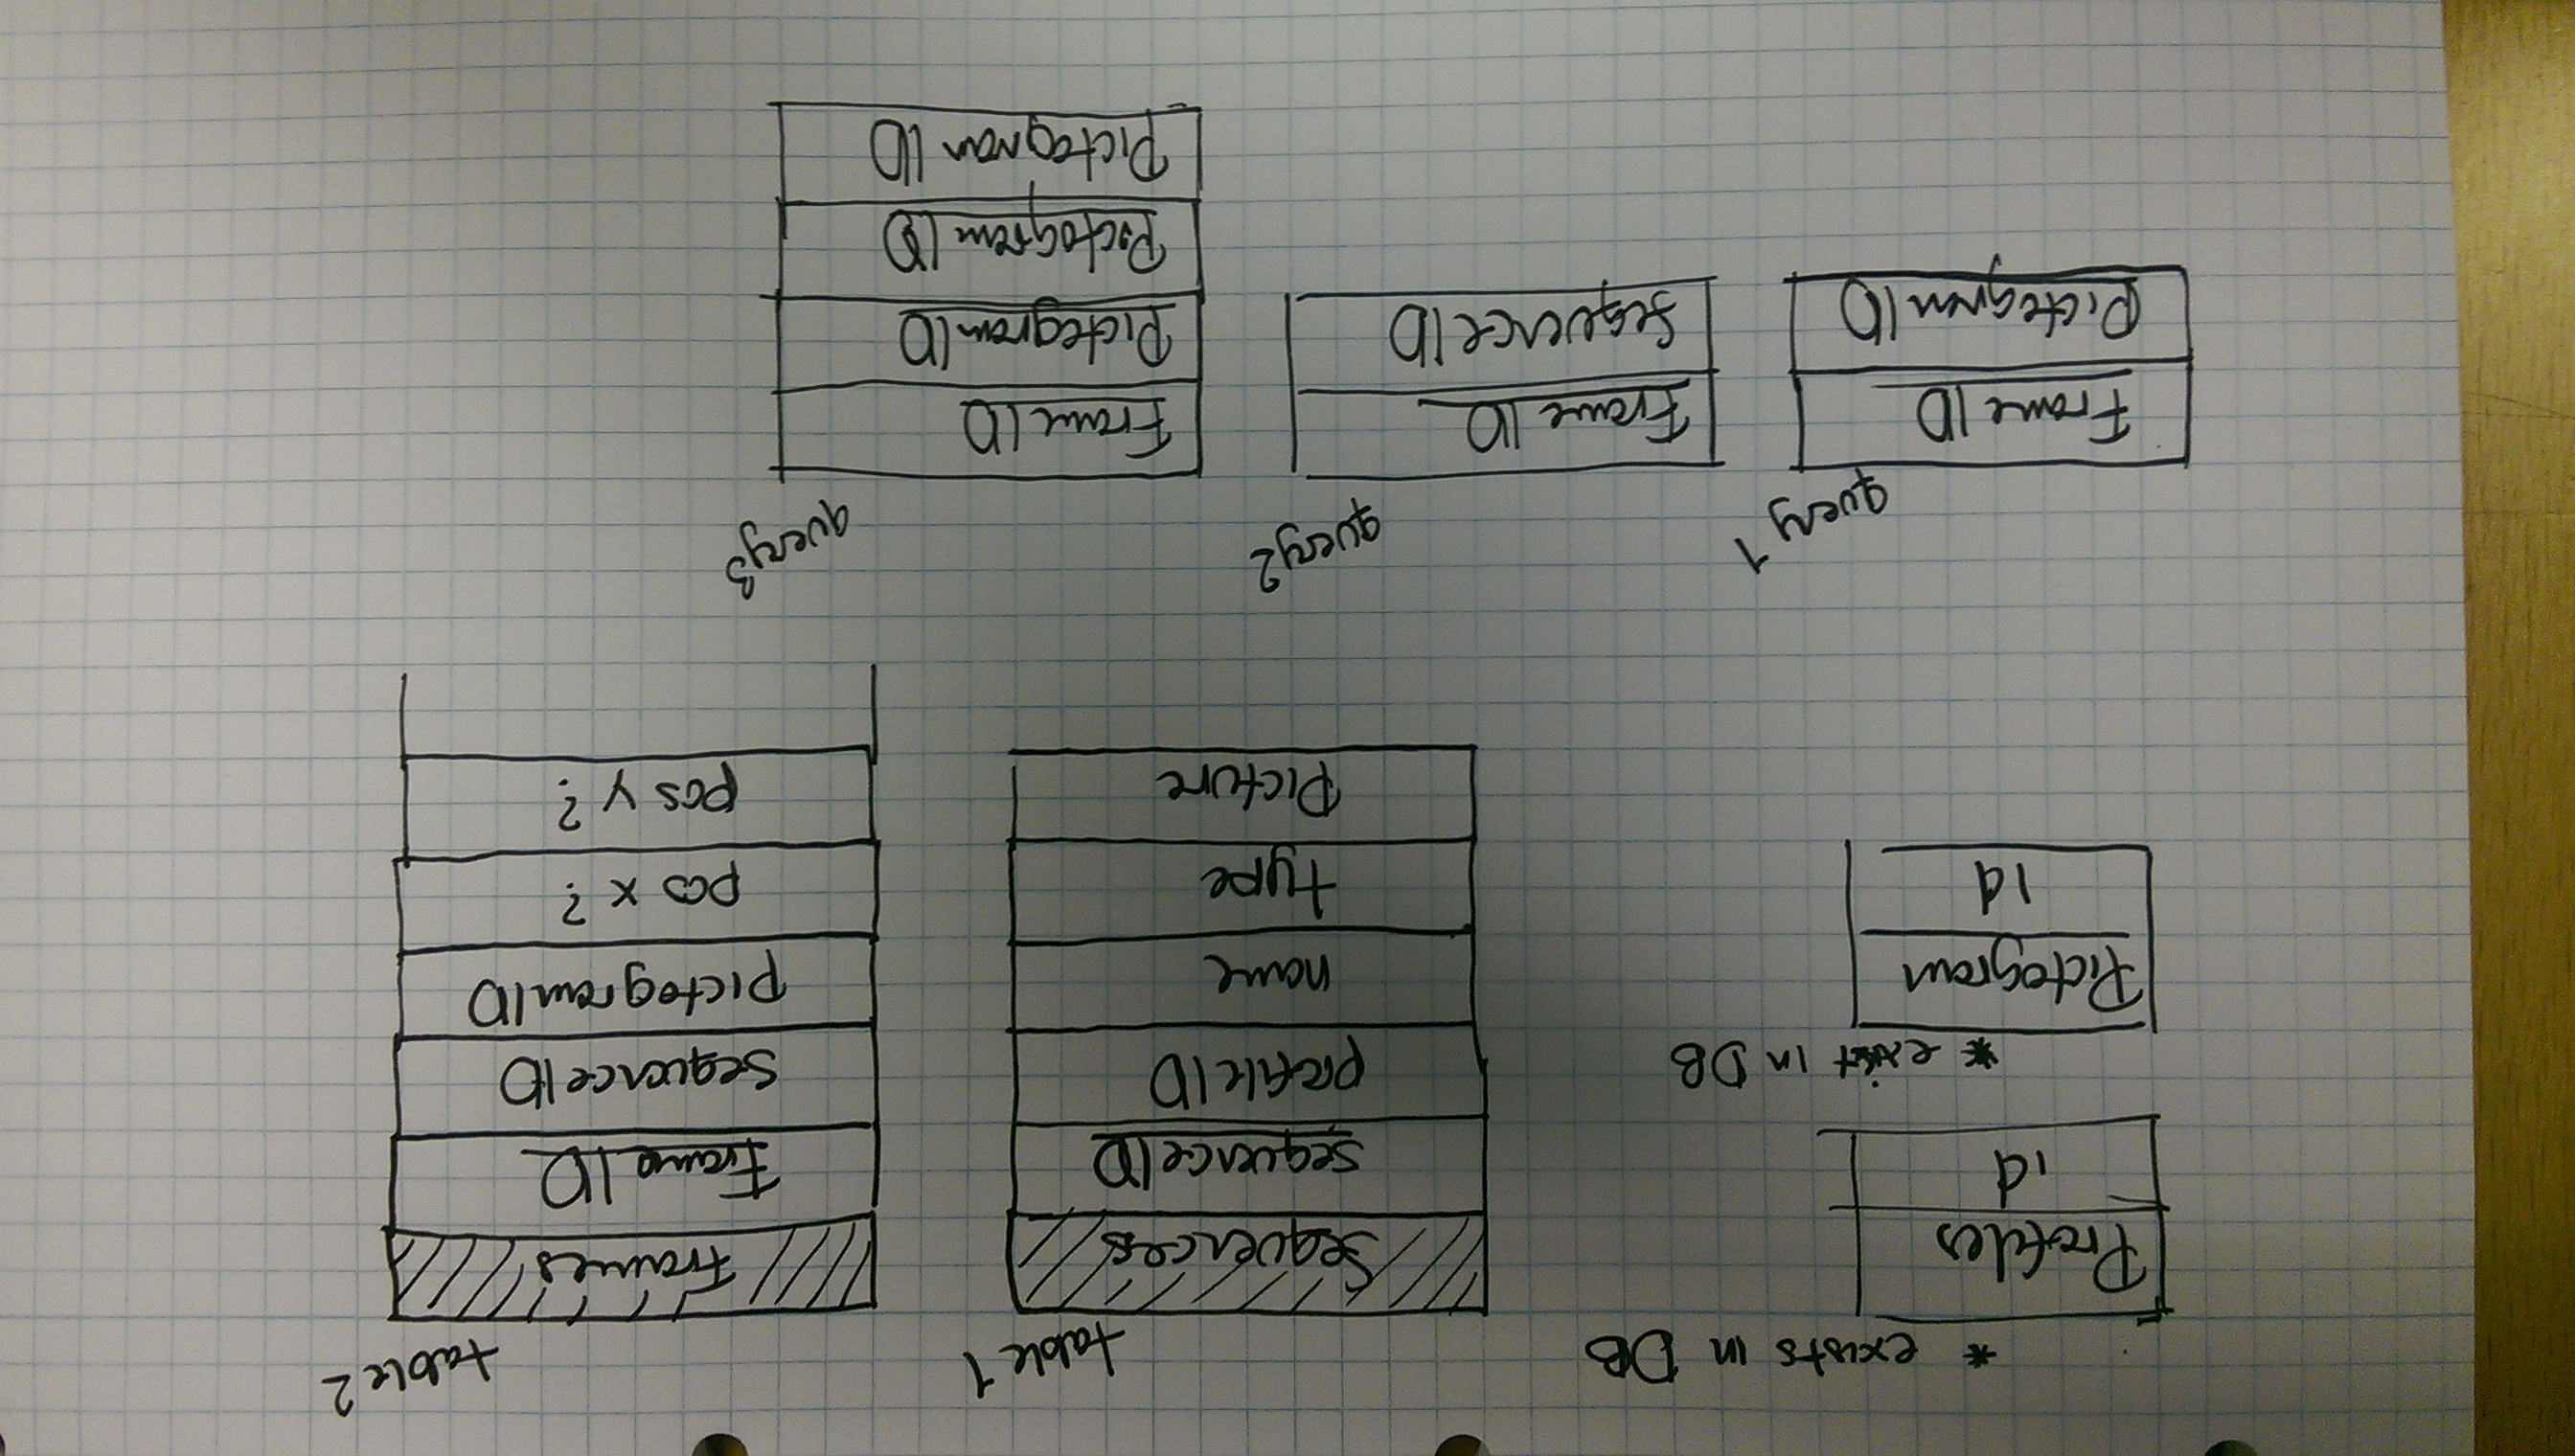
\includegraphics[width=0.7\linewidth]{Pics/ourDBdescription}
\caption{Our idea of a potential database for sequences}
\label{fig:DBdescription}
\end{figure}

As profiles and pictograms already exists in the database, these tables are not further described. We add a new sequence table that contains all of the information needed to describe a sequence from all of the groups, there is nothing really questionable here. The second table, Frames, is where the most of the magic happen. The way the pictograms/nested sequences/choices are saved in the database is they are saved to each frame. A frame can store one or more pictograms, or a nested sequenceId. This way when you are fetching a sequence from the database, you search the list of frames for frames matching the sequenceId and setting them up according to posX.\newline
\newline
The draft we submitted was quickly decided as a good baseline, but `LivsHistorier' refined it by removing the choice table, as this was possible to create through the pictogram table. We agreed that the Life-stories group will collaborate with the Database group on converting the draft to an official ER-diagram. 